\section{Integración numérica y tasas de ejecución}
\label{sec:integracion}

¿A qué frecuencia corre realmente la simulación? La pregunta surge porque la
GUI anterior se refrescaba a 50~Hz. La respuesta corta: 50~Hz es la tasa a
la que se \emph{dibuja}; la física avanza a 1~kHz con Runge--Kutta de cuarto
orden. Esta sección explica la arquitectura de relojes, justifica el
integrador y el paso, y presenta la evidencia numérica.

\subsection{Cuatro relojes, como en un autopiloto}

\begin{table}[H]
\centering
\small
\caption{Tasas de ejecución (\cod{SimConfig} y \cod{Simulation.step\_control}).}
\label{tab:tasas}
\begin{tabularx}{\textwidth}{lcX}
\toprule
Reloj & Tasa & Qué se ejecuta \\
\midrule
Física & \val{physHz}~Hz & RK4 sobre el modelo de 17 estados; \val{nsub} subpasos por periodo de control con los aceleradores retenidos (ZOH); renormalización del cuaternión; fase de los rotores; contacto con el suelo \\
Control & \val{ctrlHz}~Hz & perturbaciones, muestreo de sensores, pasa-bajos del acelerómetro y AHRS, filtros del giroscopio, filtro de navegación, lazo de actitud/tasa y mezclador. Es la tasa de \cod{TaskControlFast} del firmware ESP32 \\
Externo & \val{outerHz}~Hz & lazo vertical (modo actitud) o controlador de posición/trayectoria (modo trayectoria), uno de cada \val{nouter} periodos de control \\
Sensores lentos & 100 / 40 / 100~Hz & magnetómetro, barómetro, posición externa; mantienen el último valor entre muestras \\
Registro y GUI & 100~Hz / 50~Hz & solo lectura del estado; no afectan la simulación \\
\bottomrule
\end{tabularx}
\end{table}

La separación de un orden de magnitud entre el lazo de actitud y el de
posición es la que piden Powers, Mellinger y Kumar \cite{hb16} (pp.~317 y
321). En cada periodo de control el orden de las operaciones es: (1)
perturbaciones; (2) sensores, a partir del estado $\vect x_k$ y de su
derivada con los aceleradores del periodo anterior; (3) estimación y
filtros; (4) lazo externo, si toca; (5) lazo de actitud y mezclador, que
fijan $\sigma_k$; (6) dos pasos RK4 de 1~ms con $\sigma_k$ constante.

El paso de física es siempre un submúltiplo exacto del periodo de control,
$\Delta t_{fis}=\Delta t_{ctrl}/n_{sub}$ con $n_{sub}=\operatorname{round}(f_{fis}/f_{ctrl})$.
Si la razón pedida no es entera, la tasa de física efectiva difiere un poco
de la pedida, pero el reloj y la integración siguen sincronizados. Antes se
integraban $n_{sub}$ pasos de $1/f_{fis}$ mientras el reloj avanzaba
$1/f_{ctrl}$: con 400~Hz de control una caída libre salía un 20~\% lenta y
con 2000~Hz, el doble de rápida, y \cod{ctrl\_hz} es un parámetro que los
barridos pueden variar.

\begin{nota}[Retardo de cómputo, ESC y resolución del acelerador]
Por defecto el mando $\sigma_k$ calculado con las medidas de $t_k$ se aplica
desde $t_k$, sin el periodo de retardo de cómputo que tiene un autopiloto
real (que calcula durante el periodo y aplica al siguiente), y el ESC sigue a
$\sigma$ de forma instantánea y continua, sin frecuencia de PWM ni
protocolo. La cadena de medida sí tiene sus retardos (IMU 2~ms, más el filtro
y la retención).

La edición anterior despachaba la omisión como ``2~ms frente a los 16~ms de
retardo equivalente''. Esa comparación usa el retardo agregado de SIMC y
subestima el efecto, porque lo que importa es la fase en la frecuencia de
cruce. El guion \cod{experiments/delay\_margins.py} lo mide para el lazo de
tasa de roll con las ganancias por defecto, de dos maneras: margen de fase y
multiplicador máximo de las ganancias del lazo lineal en hover, y una
bisección en la simulación 6-DOF completa hasta que aparece una oscilación
sostenida. La \cref{tab:margenes} resume los casos. Un periodo de cómputo
quita 3.3$^\circ$ de margen de fase y baja la ganancia admisible de 5.4 a
4.3 veces; un ESC con PWM estándar de 50~Hz la deja en 2.4 veces. El motor
pesa todavía más: según la revisión externa, con $T_m=30$~ms en lugar de 20
el margen baja a 48$^\circ$. Un barrido que explore ganancias de tasa hasta
2.5 veces el valor SIMC puede encontrar, en simulación, una sintonía que en
el dron oscile.

Para estudiarlo, \cod{SimConfig} ofrece cuatro opciones desactivadas por
defecto: \cod{compute\_delay\_samples} (aplica $\sigma_{k-n}$ en lugar de
$\sigma_k$), \cod{esc\_rate\_hz} (muestreo y retención del mando a la tasa
del ESC), \cod{esc\_pulse\_delay\_s} (el valor retenido actúa un ancho de
pulso después) y \cod{throttle\_levels} (cuantiza $\sigma$ a un número finito
de niveles, como el LEDC del ESP32). Los valores por defecto conservan el
comportamiento con el que se identificaron los rezagos y se afinaron los
controladores de este documento, y así seguirán hasta tener los datos reales
del ESC y del firmware del dron (\cref{sec:limitaciones}).
\end{nota}

\begin{table}[H]
\centering
\small
\caption{Margen del lazo de tasa de roll del PAE-X450 con las ganancias por
defecto y distintas cadenas de actuación
(\cod{experiments/results/delay\_margins/}). Cruce en 4.7~Hz en todos los
casos. Ganancia máxima: factor común sobre $K_p$, $K_i$ y $K_d$ de tasa antes
de la inestabilidad, en el lazo lineal y en la simulación completa. Las
filas son escenarios, no mediciones del dron.}
\label{tab:margenes}
\begin{tabular}{lcccc}
\toprule
Cadena de actuación & MF [$^\circ$] & MG [dB] & Gan. máx. (lineal) & Gan. máx. (6-DOF) \\
\midrule
Continua, sin cómputo (por defecto) & 58.7 & 14.6 & 5.39 & 4.91 \\
+1 periodo de cómputo (2~ms) & 55.4 & 12.7 & 4.30 & 3.91 \\
+2 periodos de cómputo (4~ms) & 52.0 & 11.1 & 3.60 & 3.22 \\
ESC 400~Hz + 1 periodo & 53.2 & 11.7 & 3.84 & 3.67 \\
ESC 400~Hz + 1 periodo + pulso 1.5~ms & 50.7 & 10.6 & 3.40 & 3.22 \\
ESC 50~Hz + pulso 1.5~ms & 39.6 & 7.8 & 2.44 & 2.25 \\
\bottomrule
\end{tabular}
\end{table}

\subsection{Los integradores}

Con la entrada constante en el paso, $\dot{\vect x}=f(\vect x)$, el código
(\cod{dynamics.rk4\_step}) implementa Runge--Kutta clásico:
\begin{equation}
\begin{gathered}
\vect k_1=f(\vect x_n),\quad
\vect k_2=f\!\big(\vect x_n+\tfrac{h}{2}\vect k_1\big),\quad
\vect k_3=f\!\big(\vect x_n+\tfrac{h}{2}\vect k_2\big),\quad
\vect k_4=f(\vect x_n+h\vect k_3),\\
\vect x_{n+1}=\vect x_n+\tfrac{h}{6}\big(\vect k_1+2\vect k_2+2\vect k_3+\vect k_4\big),
\end{gathered}
\label{eq:rk4}
\end{equation}
con error local $O(h^5)$ y global $O(h^4)$ \cite{hairer93}. Euler explícito,
$\vect x_{n+1}=\vect x_n+h f(\vect x_n)$ (global $O(h)$), se conserva solo
para comparar (\cod{SimConfig.integrator="euler"}).

\paragraph{Estabilidad.} El modo más rápido del modelo en lazo abierto es el
del motor, $\lambda=-1/T_m=-50$~s$^{-1}$ (\cref{tab:jac}). A 1~kHz,
$h\lambda=-0.05$. Euler es estable para $h\lambda\in(-2,0)$, o sea
$h<2T_m=40$~ms; RK4, en el eje real, para $h\lambda>-2.785$, o sea
$h<55.7$~ms. La estabilidad numérica no es la restricción que fija el paso:
lo son la exactitud y la necesidad de que la física sea más rápida que el
lazo de control que la observa. El NMPC de la \cref{sec:posicion}, con paso de
predicción de 50~ms, sí queda cerca de ese límite en su modelo interno
($\Delta t_{pred}/\tau_T=2.6$), y por eso integra exactamente sus estados de
rezago.

\paragraph{La vibración no necesita física más rápida.} El tono de 177~Hz
podría parecer un argumento para integrar más rápido. No lo es: la fase de
cada rotor se avanza analíticamente, $\varphi_i\leftarrow\varphi_i+\Omega_i h$,
y el sensor la evalúa en los instantes de muestreo. El tono que ve la IMU es
exacto para cualquier paso de física.

\subsection{Evidencia numérica}

\paragraph{Orden de convergencia.} El bloque E integra durante 1~s una
maniobra no lineal genérica (velocidad de $(3,-2,1)$~m/s, actitud y velocidad
angular no nulas, rotores desbalanceados, aceleradores fijos distintos) con
pasos de 8~ms a 0.25~ms, y compara con una solución de referencia RK4 de
$h=25~\mu$s. Se comprobó que a lo largo de la referencia ninguna componente
de $\vect v_B$ ni de $\vect\omega$ cruza cero (mínimo $|\cdot|$ =
\val{minVb}): las funciones $x|x|$ del arrastre no tienen ``esquinas'' en el
intervalo, condición para que RK4 alcance su orden.

\begin{figure}[H]
\centering
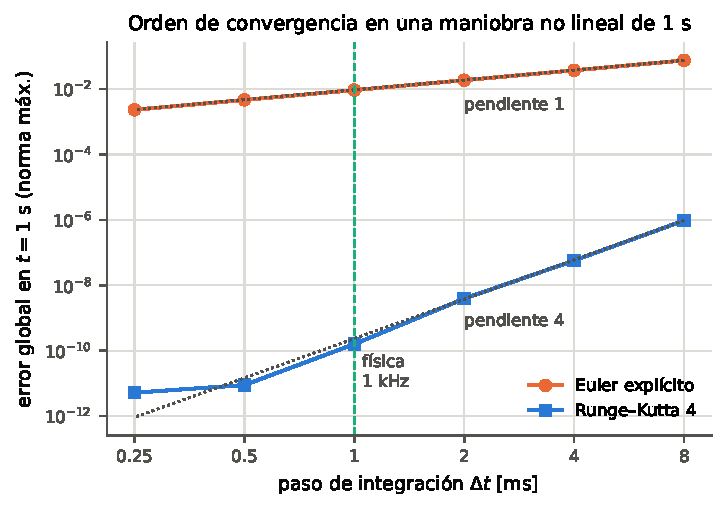
\includegraphics[width=0.72\textwidth]{convergencia_integradores.pdf}
\caption{Error global en $t=1$~s frente al paso. Pendientes ajustadas: Euler
\val{ordEuler}, RK4 \val{ordRK} (pares sucesivos: \val{ordRKpares}). El último
punto de RK4 toca el piso de redondeo ($\approx$\val{errRKfloor}).}
\label{fig:conv}
\end{figure}

Las pendientes medidas, \val{ordEuler} y \val{ordRK}, son las teóricas 1 y 4.
Al paso de 1~ms el error de RK4 es \val{errRK1ms}; un Euler explícito con el paso
de 2~ms de la 2.ª edición tiene \val{errEu2ms}, ocho órdenes de magnitud más.

\paragraph{Conservación en rotación libre.} Sin arrastre, sin
amortiguamiento y con los rotores parados, el cuerpo rígido conserva la
energía $E=\tfrac12\vect\omega\T J\vect\omega$ y el momento angular en el
marco inercial, $\vect L_E=\R J\vect\omega$. Son invariantes exactos que
ningún integrador de paso fijo genérico conserva por construcción; medir su
deriva es una prueba independiente. Además, el PAE-X450 cumple
$J_{yy}<J_{xx}<J_{zz}$, así que un giro alrededor de $x$ es un giro
alrededor del eje \emph{intermedio}, inestable (efecto Dzhanibekov o
teorema de la raqueta de tenis \cite{landau76}). Linealizando las
ecuaciones de Euler alrededor de $\vect\omega=(\omega_0,0,0)$, las
perturbaciones crecen con tasa
\begin{equation}
\lambda=\omega_0\sqrt{\frac{(J_{xx}-J_{yy})(J_{zz}-J_{xx})}{J_{yy}J_{zz}}}=\val{dzLam}~\text{s}^{-1}\quad(\omega_0=20~\text{rad/s}).
\label{eq:dzh}
\end{equation}
Con perturbaciones iniciales de $10^{-3}$~rad/s, la primera inversión se
espera hacia $\ln(20/1.4\times10^{-3})/\lambda\approx\val{dzEst}$~s; la
simulación la da a los \val{dzFirst}~s y muestra \val{dzFlips} inversiones de
$\omega_x$ en 40~s (\cref{fig:dzh}). Los ejes estables sí lo son: girando
alrededor de $z$ (inercia máxima) o de $y$ (mínima), las componentes
transversales se quedan por debajo de \val{stabZ} y \val{stabY}~rad/s en
10~s.

\begin{figure}[H]
\centering
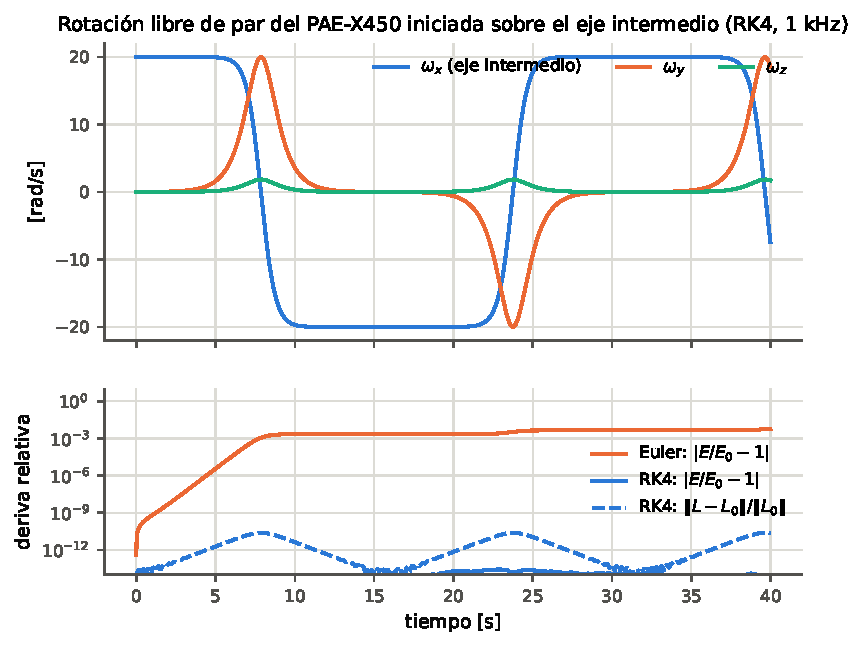
\includegraphics[width=0.8\textwidth]{dzhanibekov_conservacion.pdf}
\caption{Rotación libre iniciada sobre el eje intermedio. Arriba: inversiones
periódicas de $\omega_x$. Abajo: deriva relativa de la energía y del momento
angular inercial con RK4 y con Euler a 1~kHz.}
\label{fig:dzh}
\end{figure}

Con RK4 a 1~kHz la deriva máxima en 40~s es \val{freeRKE} en energía y
\val{freeRKL} en momento angular; con Euler al mismo paso, \val{freeEuE} y
\val{freeEuL}. La diferencia muestra qué tan engañoso puede ser Euler en una
simulación larga: inyecta energía, y lo hace justo en las fases rápidas de la
inversión.

\paragraph{Exactitud en lazo cerrado.} La prueba que más le importa al
usuario es si la frecuencia de física cambia los resultados del simulador
completo. El bloque E corre 3~s con escalones de roll de $\pm15^\circ$
(estimador ideal, sensores sin ruido, controlador a 500~Hz) con física a
16~kHz como referencia y compara:

\begin{table}[H]
\centering
\small
\caption{Error máximo frente a la referencia de 16~kHz en lazo cerrado.}
\label{tab:cl}
\begin{tabular}{lcc}
\toprule
Integrador y tasa de física & roll [$^\circ$] & posición lateral $y$ [m] \\
\midrule
RK4, 1000~Hz (por defecto) & \val{clRKmilphi} & \val{clRKmily} \\
RK4, 500~Hz & \val{clRKquiphi} & \val{clRKquiy} \\
Euler, 1000~Hz & \val{clEumilphi} & \val{clEumily} \\
Euler, 500~Hz (2.ª edición) & \val{clEuquiphi} & \val{clEuquiy} \\
\bottomrule
\end{tabular}
\end{table}

Con RK4 la física a 1~kHz es indistinguible de la de 16~kHz (error de
millonésimas de grado) y la de 500~Hz también bastaría; los 1000~Hz se
eligieron por margen, a un costo bajo. Euler a 500~Hz se separa
\val{clEuquiphi}$^\circ$ en roll y \val{clEuquiy}~m en posición lateral en
tres segundos: no es catastrófico, pero es del orden
de los efectos que se quieren estudiar (errores de estimación de décimas de
grado, errores de seguimiento de centímetros), y crece con la duración.

\paragraph{Costo.} Con el estimador por defecto (\val{estDef}), el simulador
completo corre a unas \val{rtf} veces el tiempo real en un núcleo (bloque L;
medido con otro proceso pesado compartiendo la CPU), suficiente para
barridos de cientos de corridas y para la GUI en tiempo real.
